\section{Methodology}\label{sec:methodology}

The proposed method simulates the natural degradation of printed icons on textured surfaces by blending an icon with a randomly selected paper texture. The approach ensures that the icon's appearance is influenced by the physical characteristics of the paper, such as darkness, creases, and smudges, to create realistic augmentations.

\subsection{Paper Texture Analysis and Degradation}

To replicate realistic degradation, we collected various textured paper sheets with different levels of wear. These textures exhibit characteristics such as darkness, creasing, and smudging, which influence how the icon blends with the background.

Darker paper reduces contrast and absorbs more light, affecting the visibility of the printed icon. As shown in Figure~\ref{fig:dark-paper}, varying levels of darkness impact the overall perception of detail, requiring adjustments to the blending process to ensure proper integration.

\begin{figure}
    \centering
    \begin{subfigure}{0.3\textwidth}
        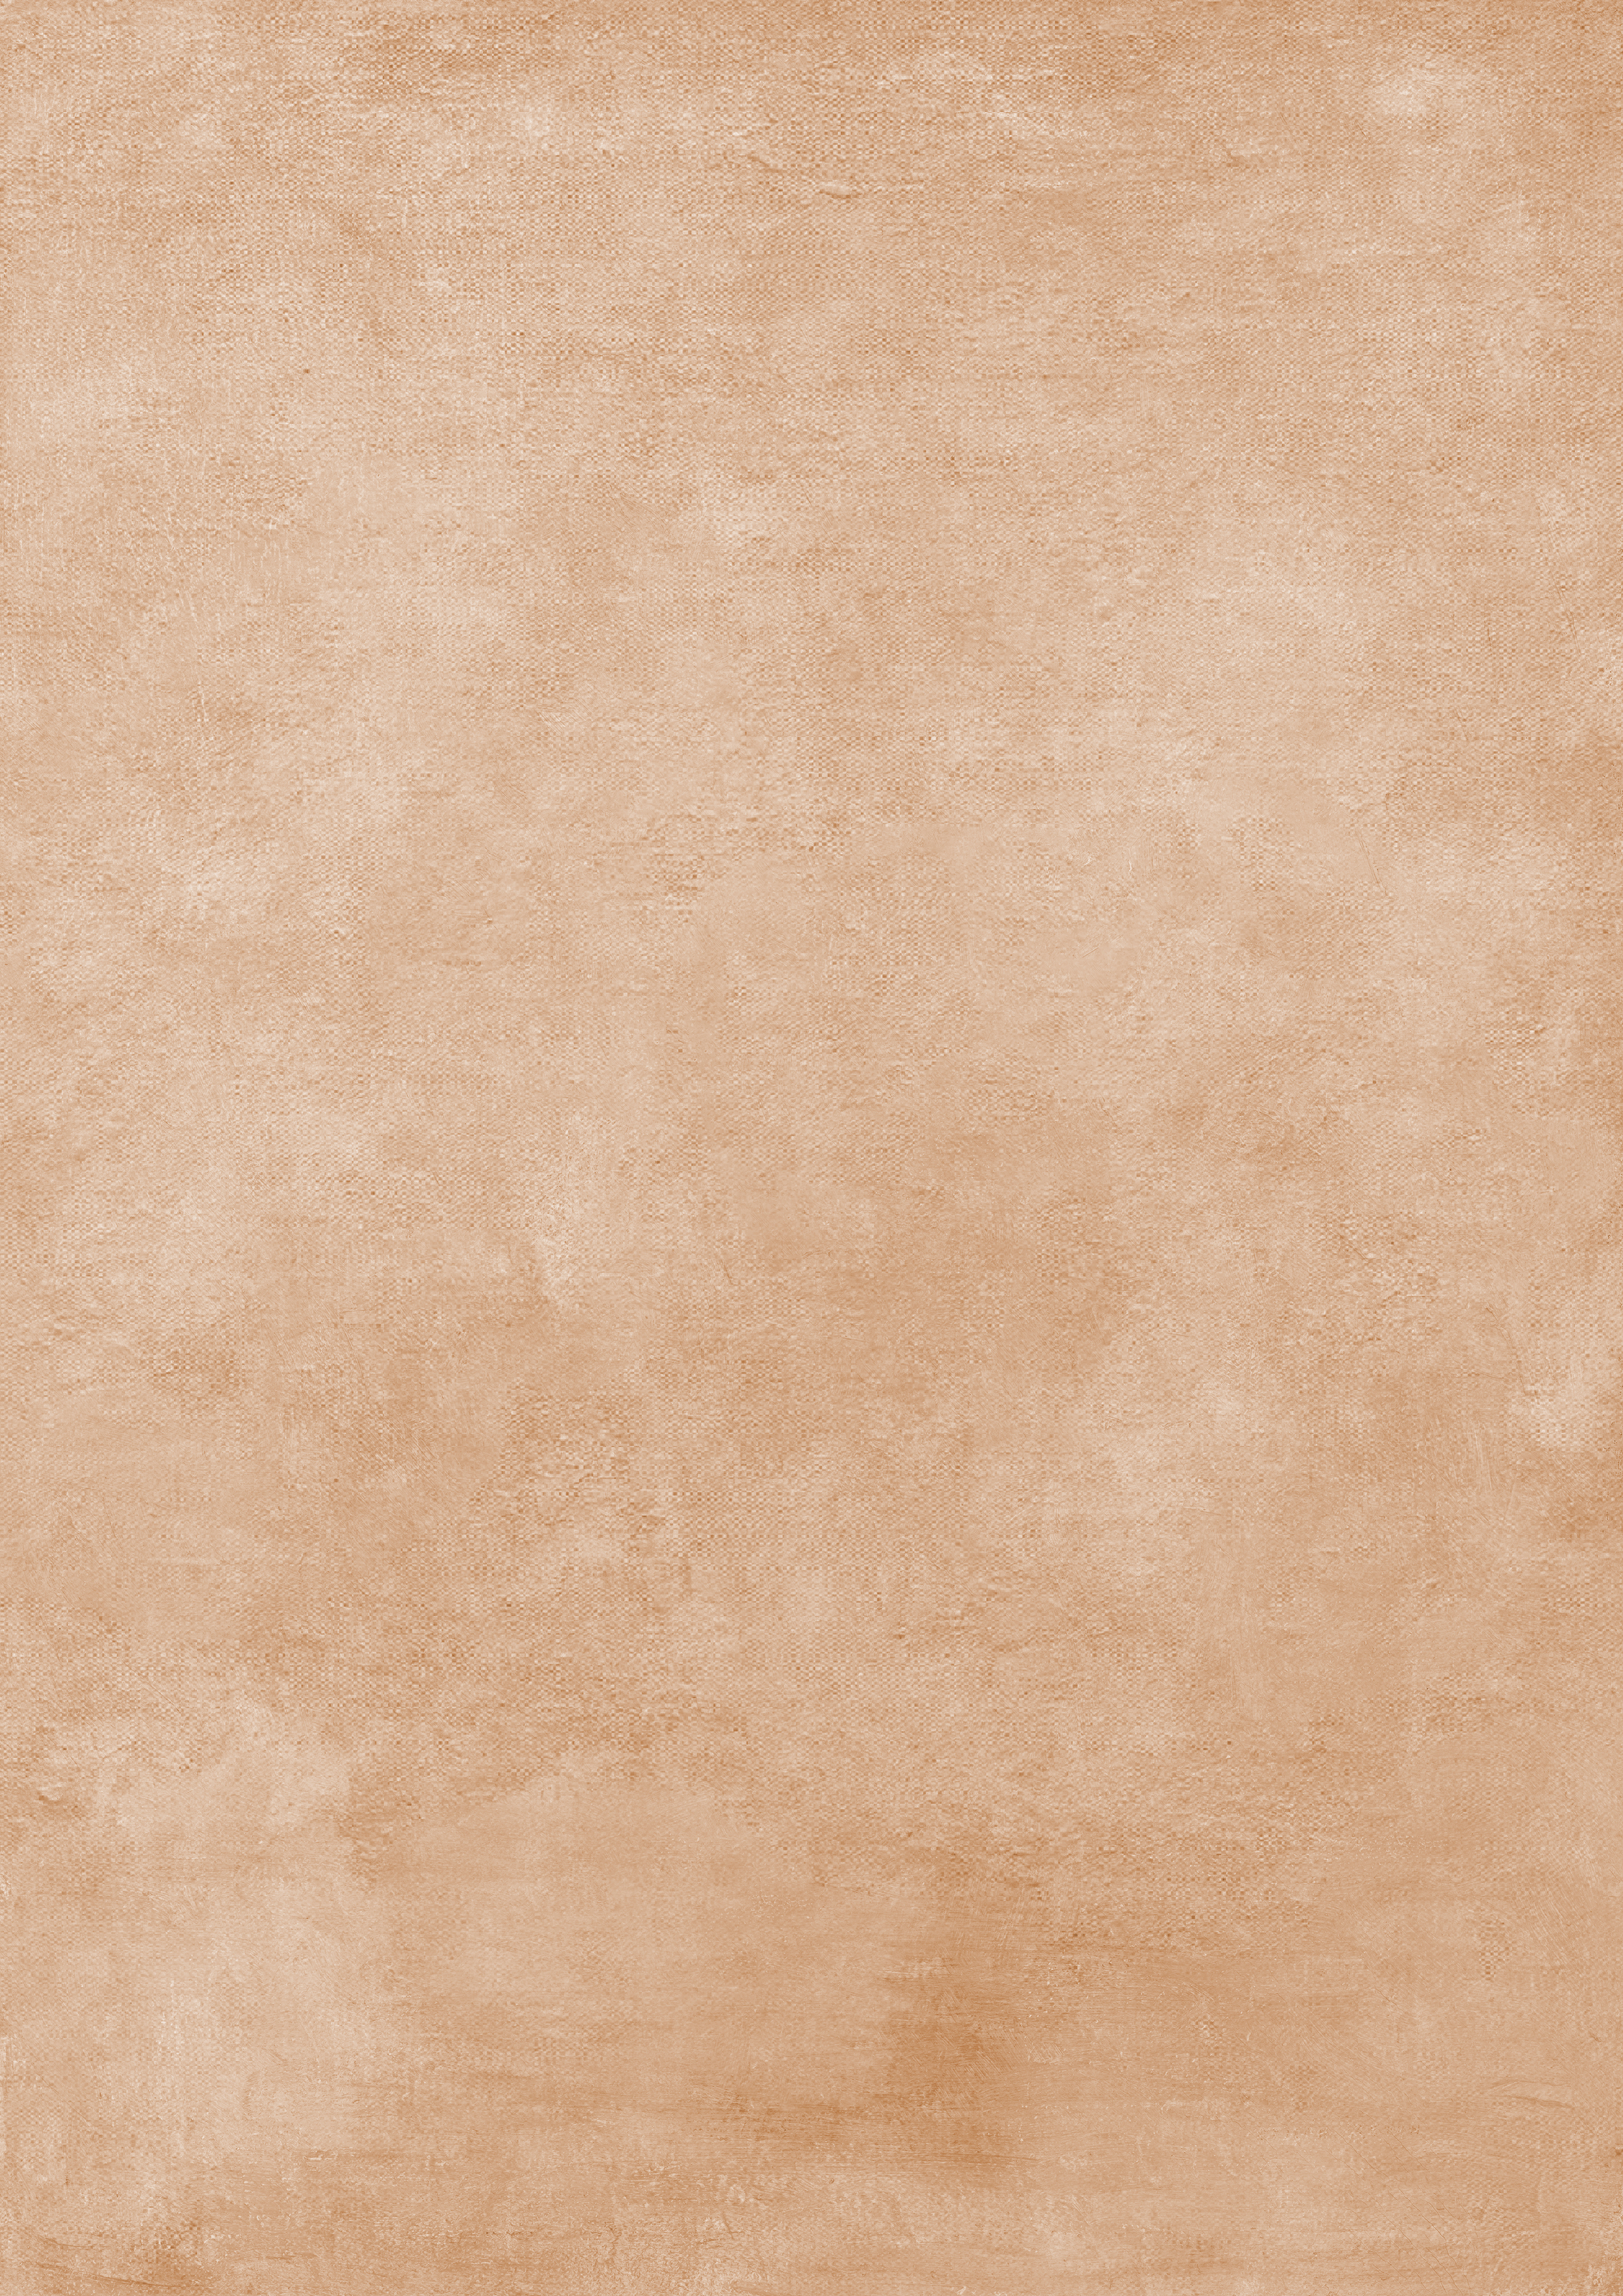
\includegraphics[width=\textwidth]{images/006.jpg}
        \caption{Lightly darkened.}
    \end{subfigure}
    \begin{subfigure}{0.3\textwidth}
        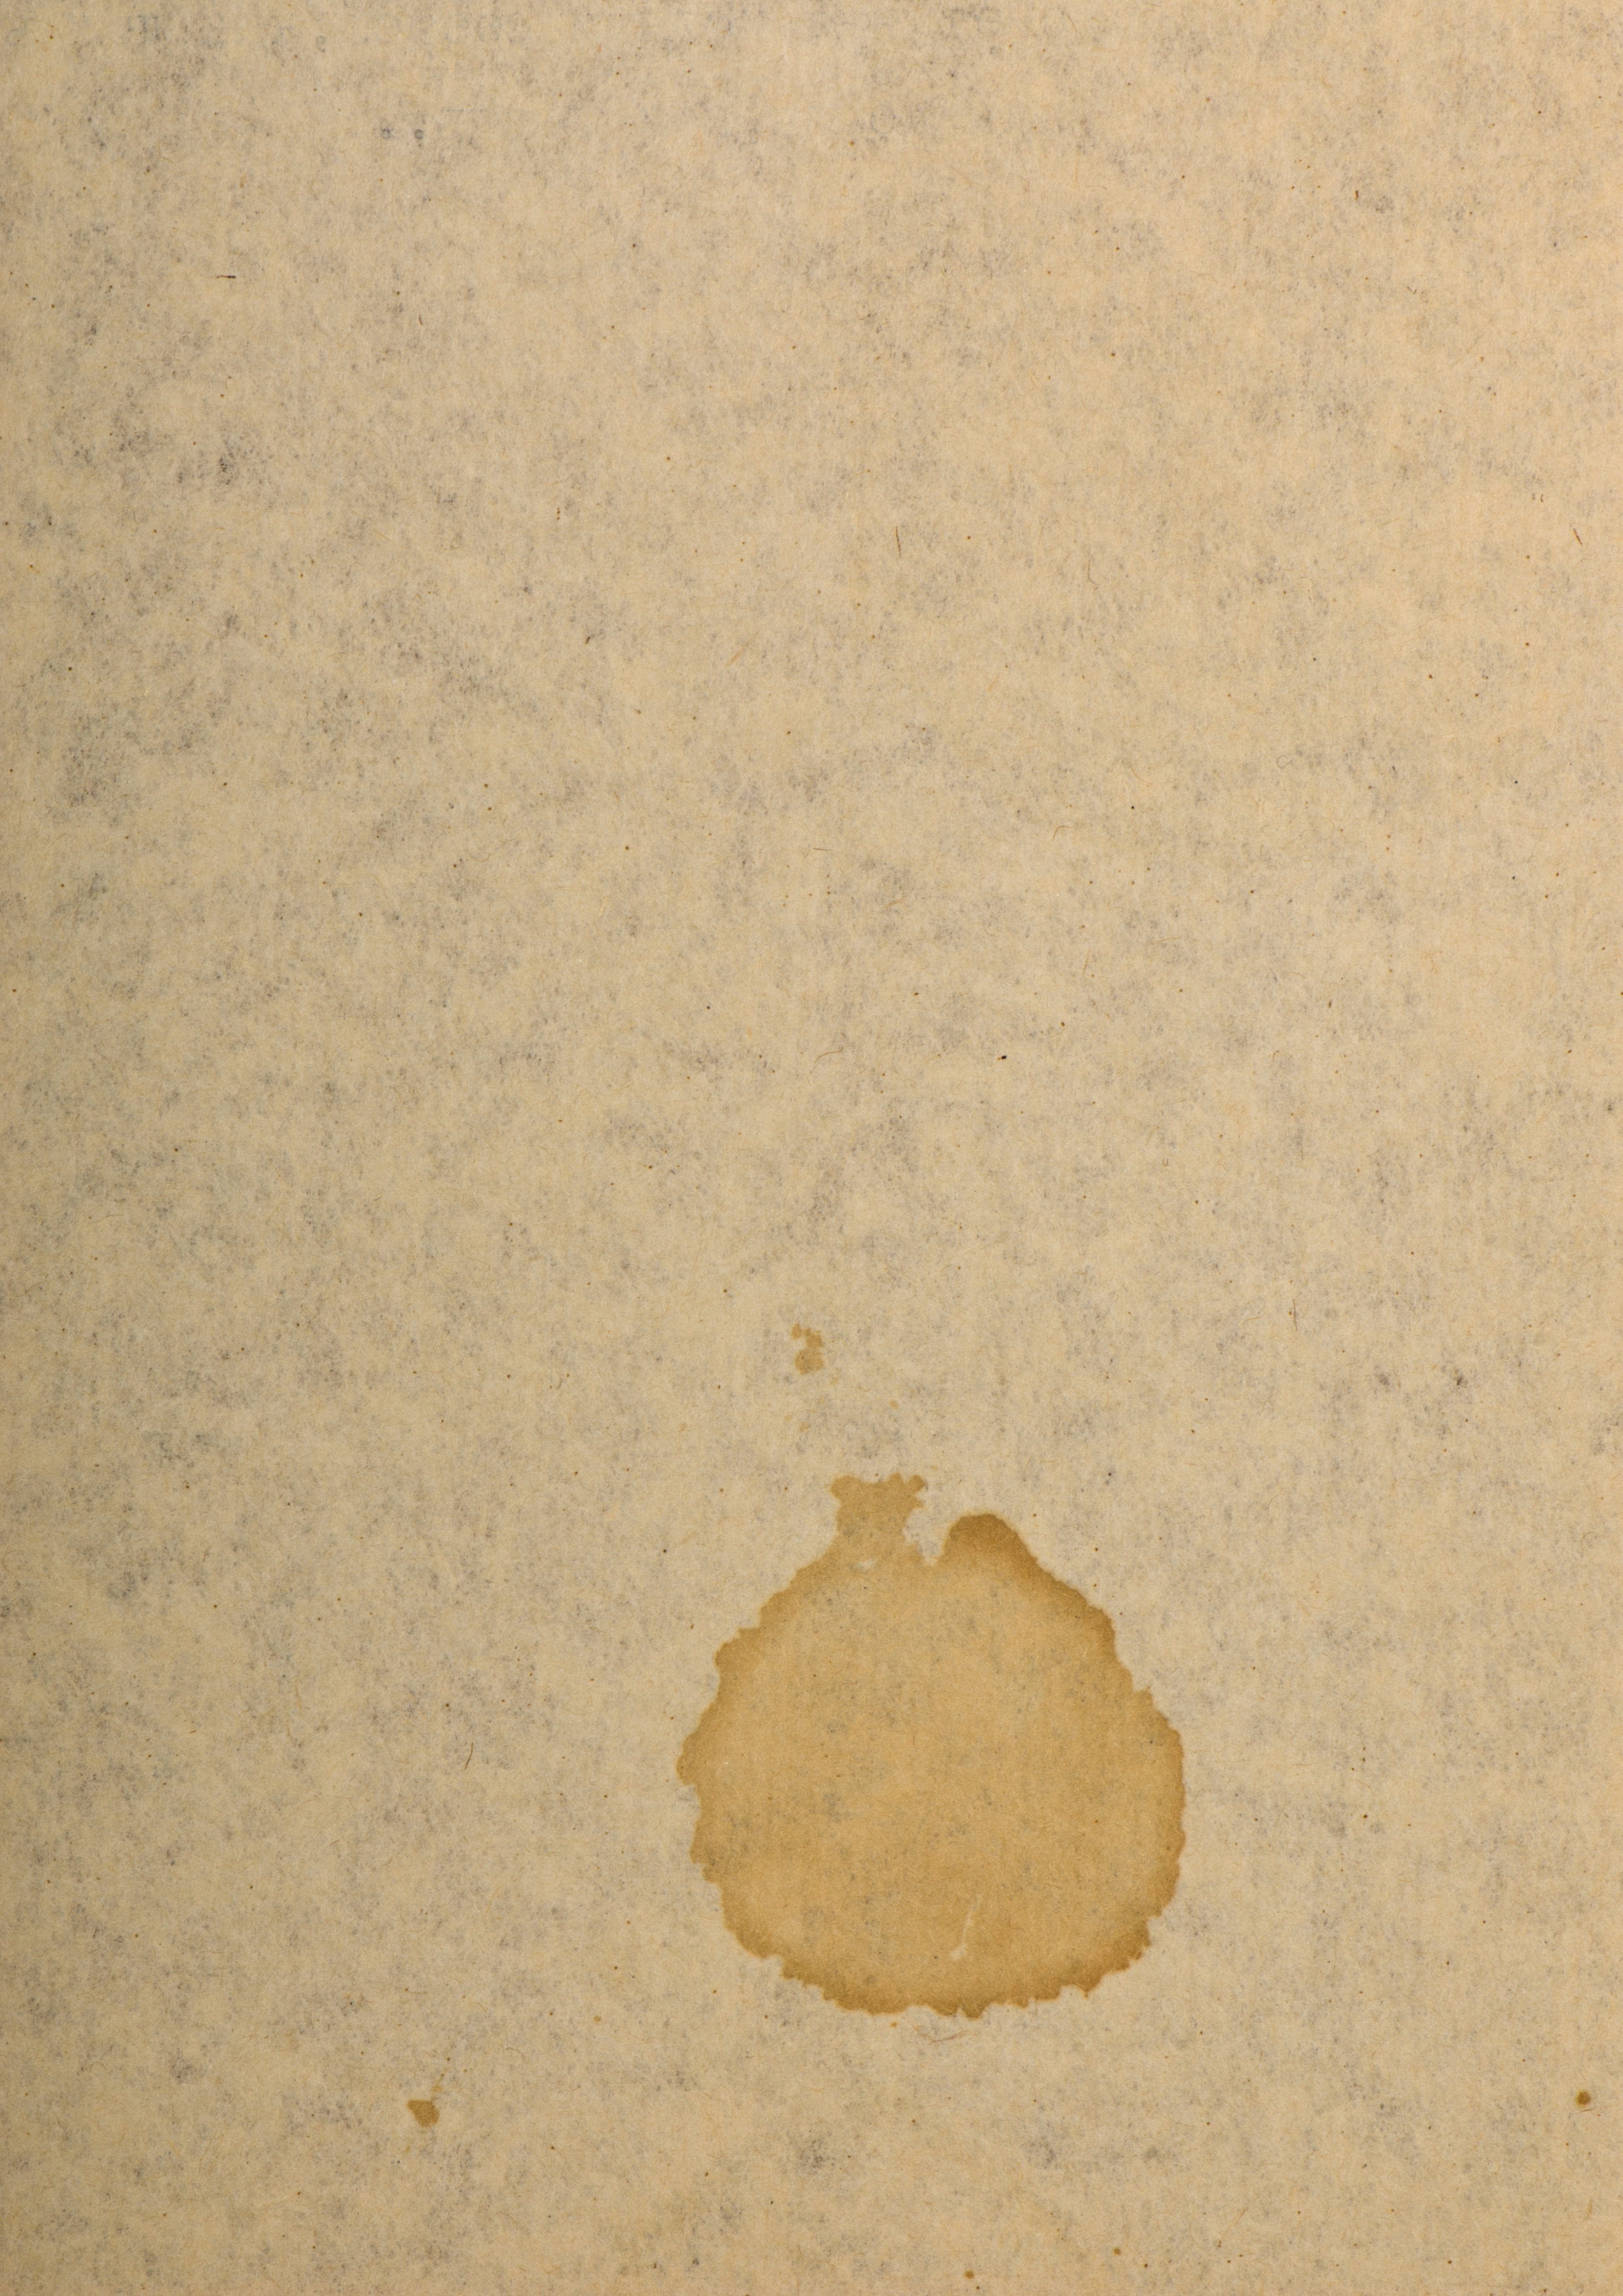
\includegraphics[width=\textwidth]{images/007.jpg}
        \caption{Moderately darkened.}
    \end{subfigure}
    \begin{subfigure}{0.3\textwidth}
        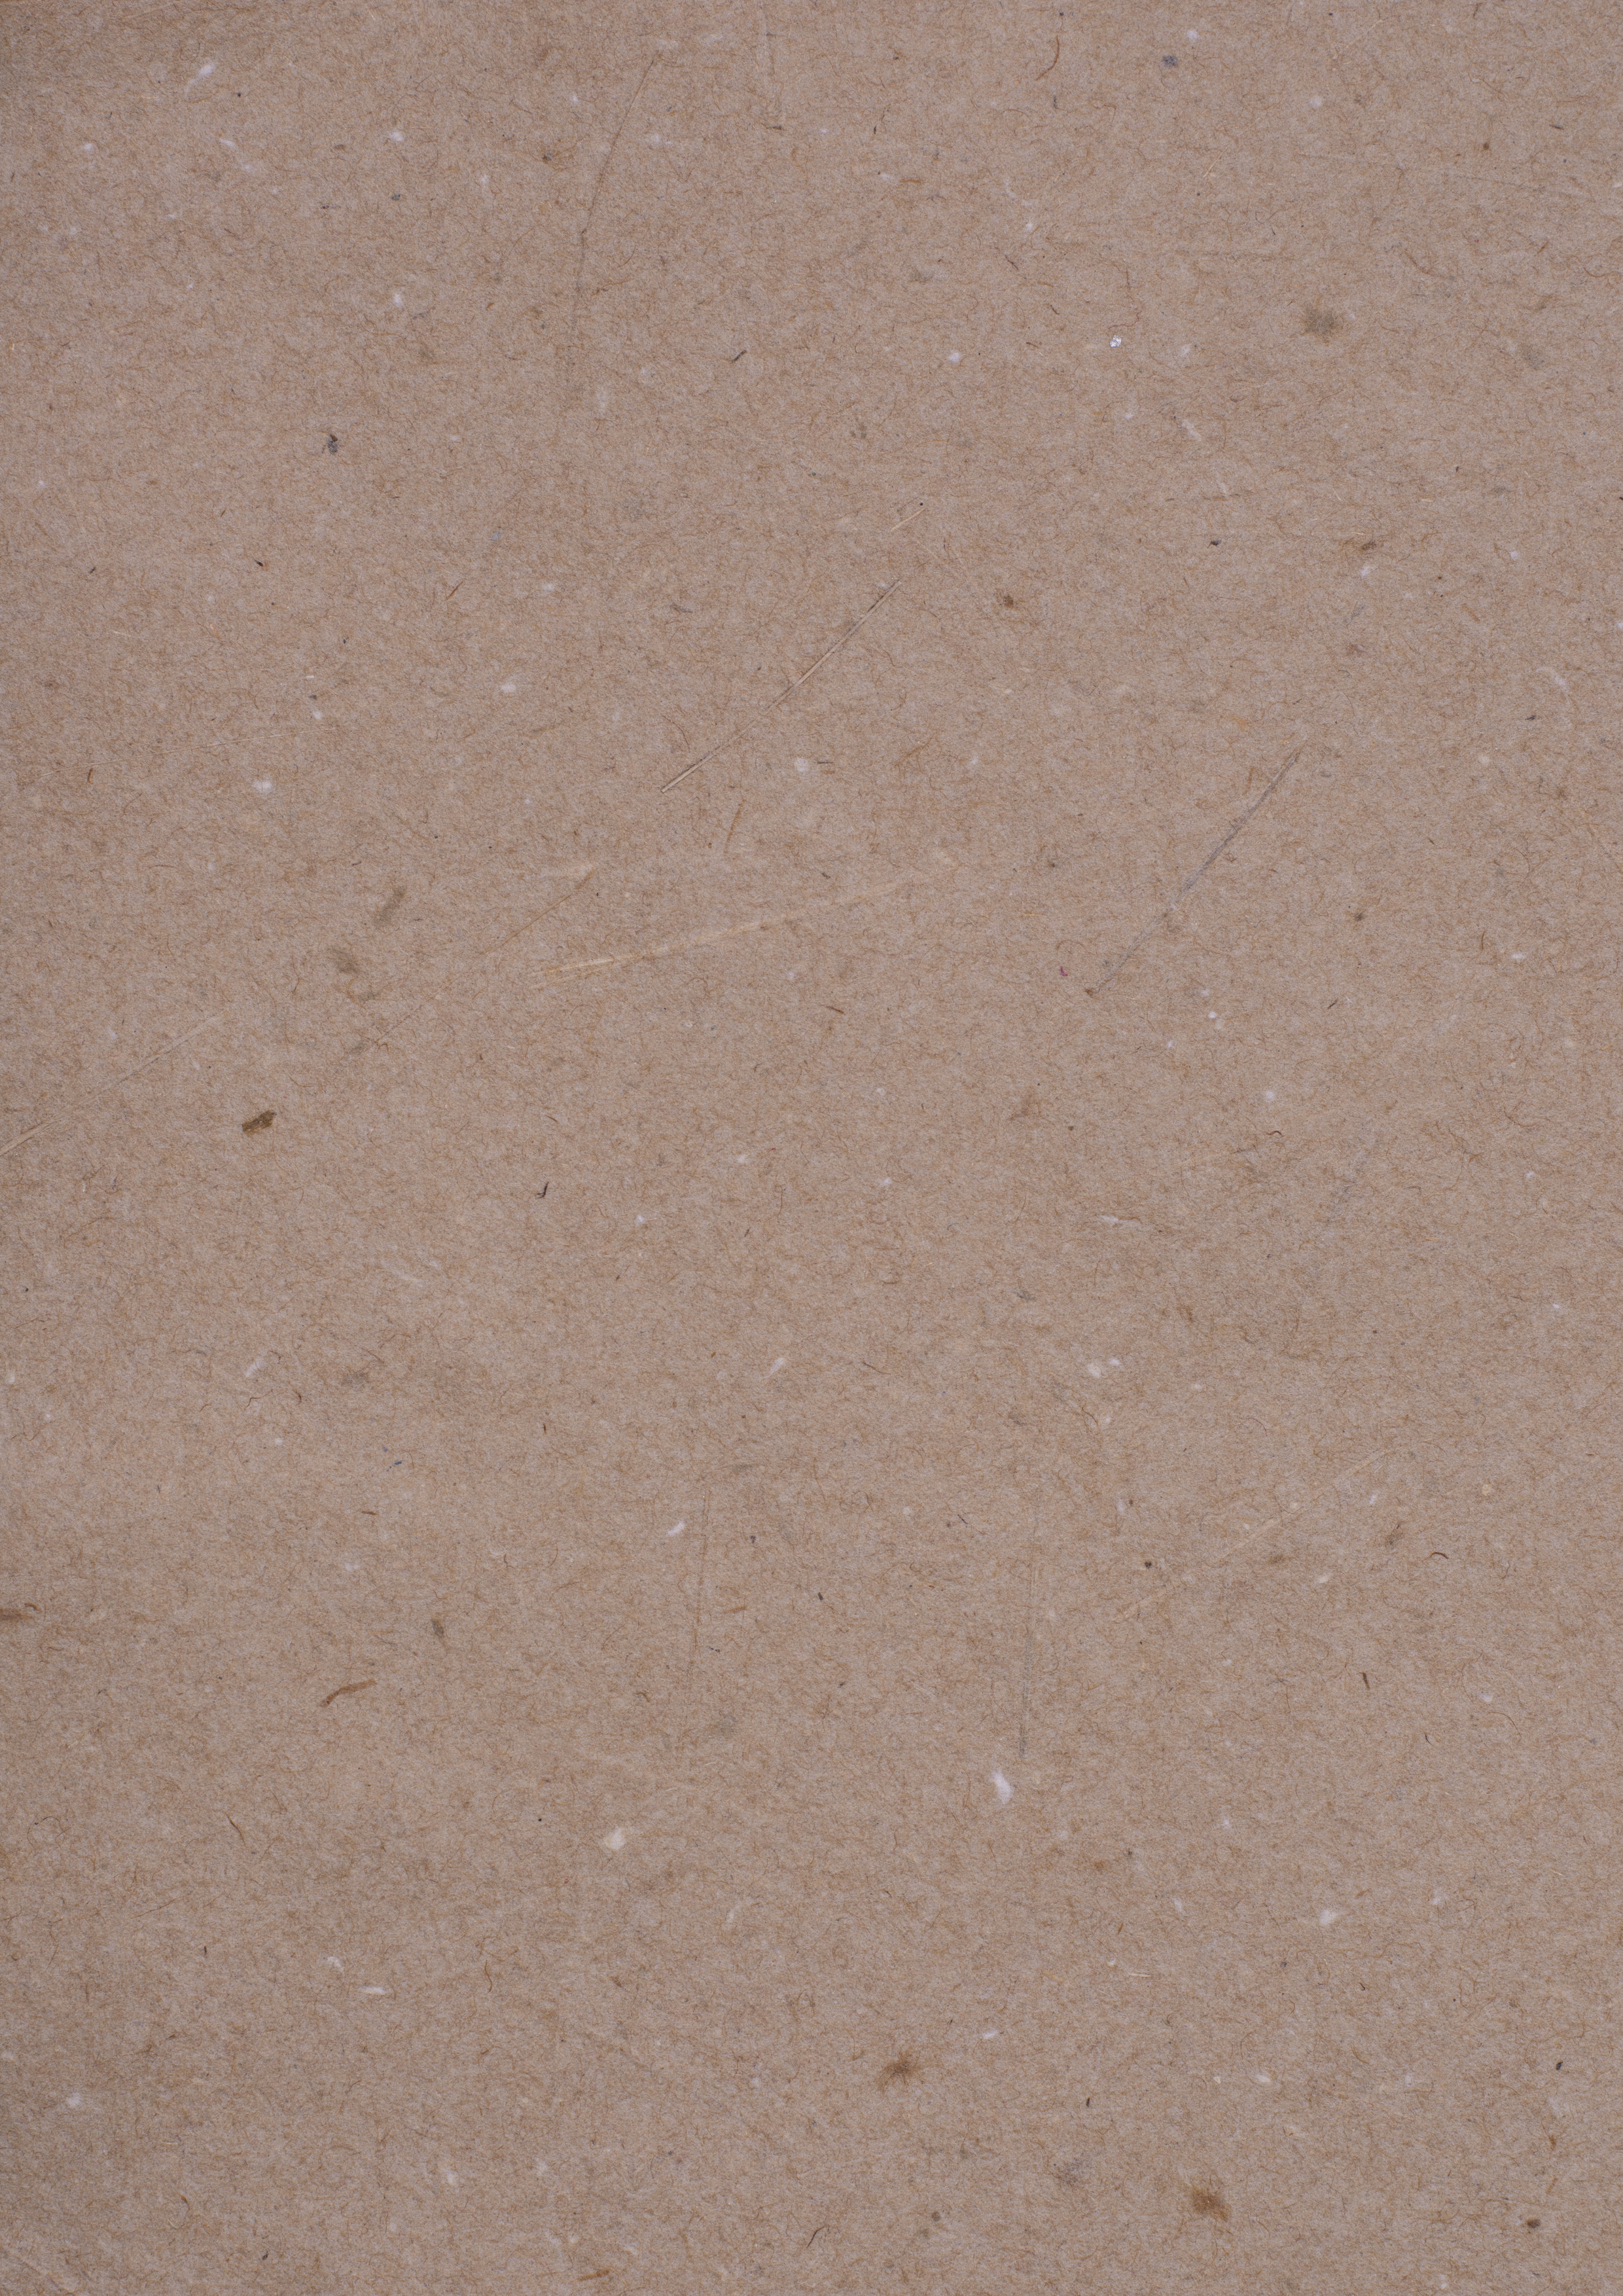
\includegraphics[width=\textwidth]{images/008.jpg}
        \caption{Heavily darkened.}
    \end{subfigure}
    \caption{Examples of paper with increasing levels of darkness.}\label{fig:dark-paper}
\end{figure}

Creased and scratched paper introduces irregular surface distortions, altering the way printed elements interact with the texture. As shown in Figure~\ref{fig:creased-paper}, creases and scratches disrupt the uniformity of the surface, affecting how elements blend with the background.

\begin{figure}
    \centering
    \begin{subfigure}{0.3\textwidth}
        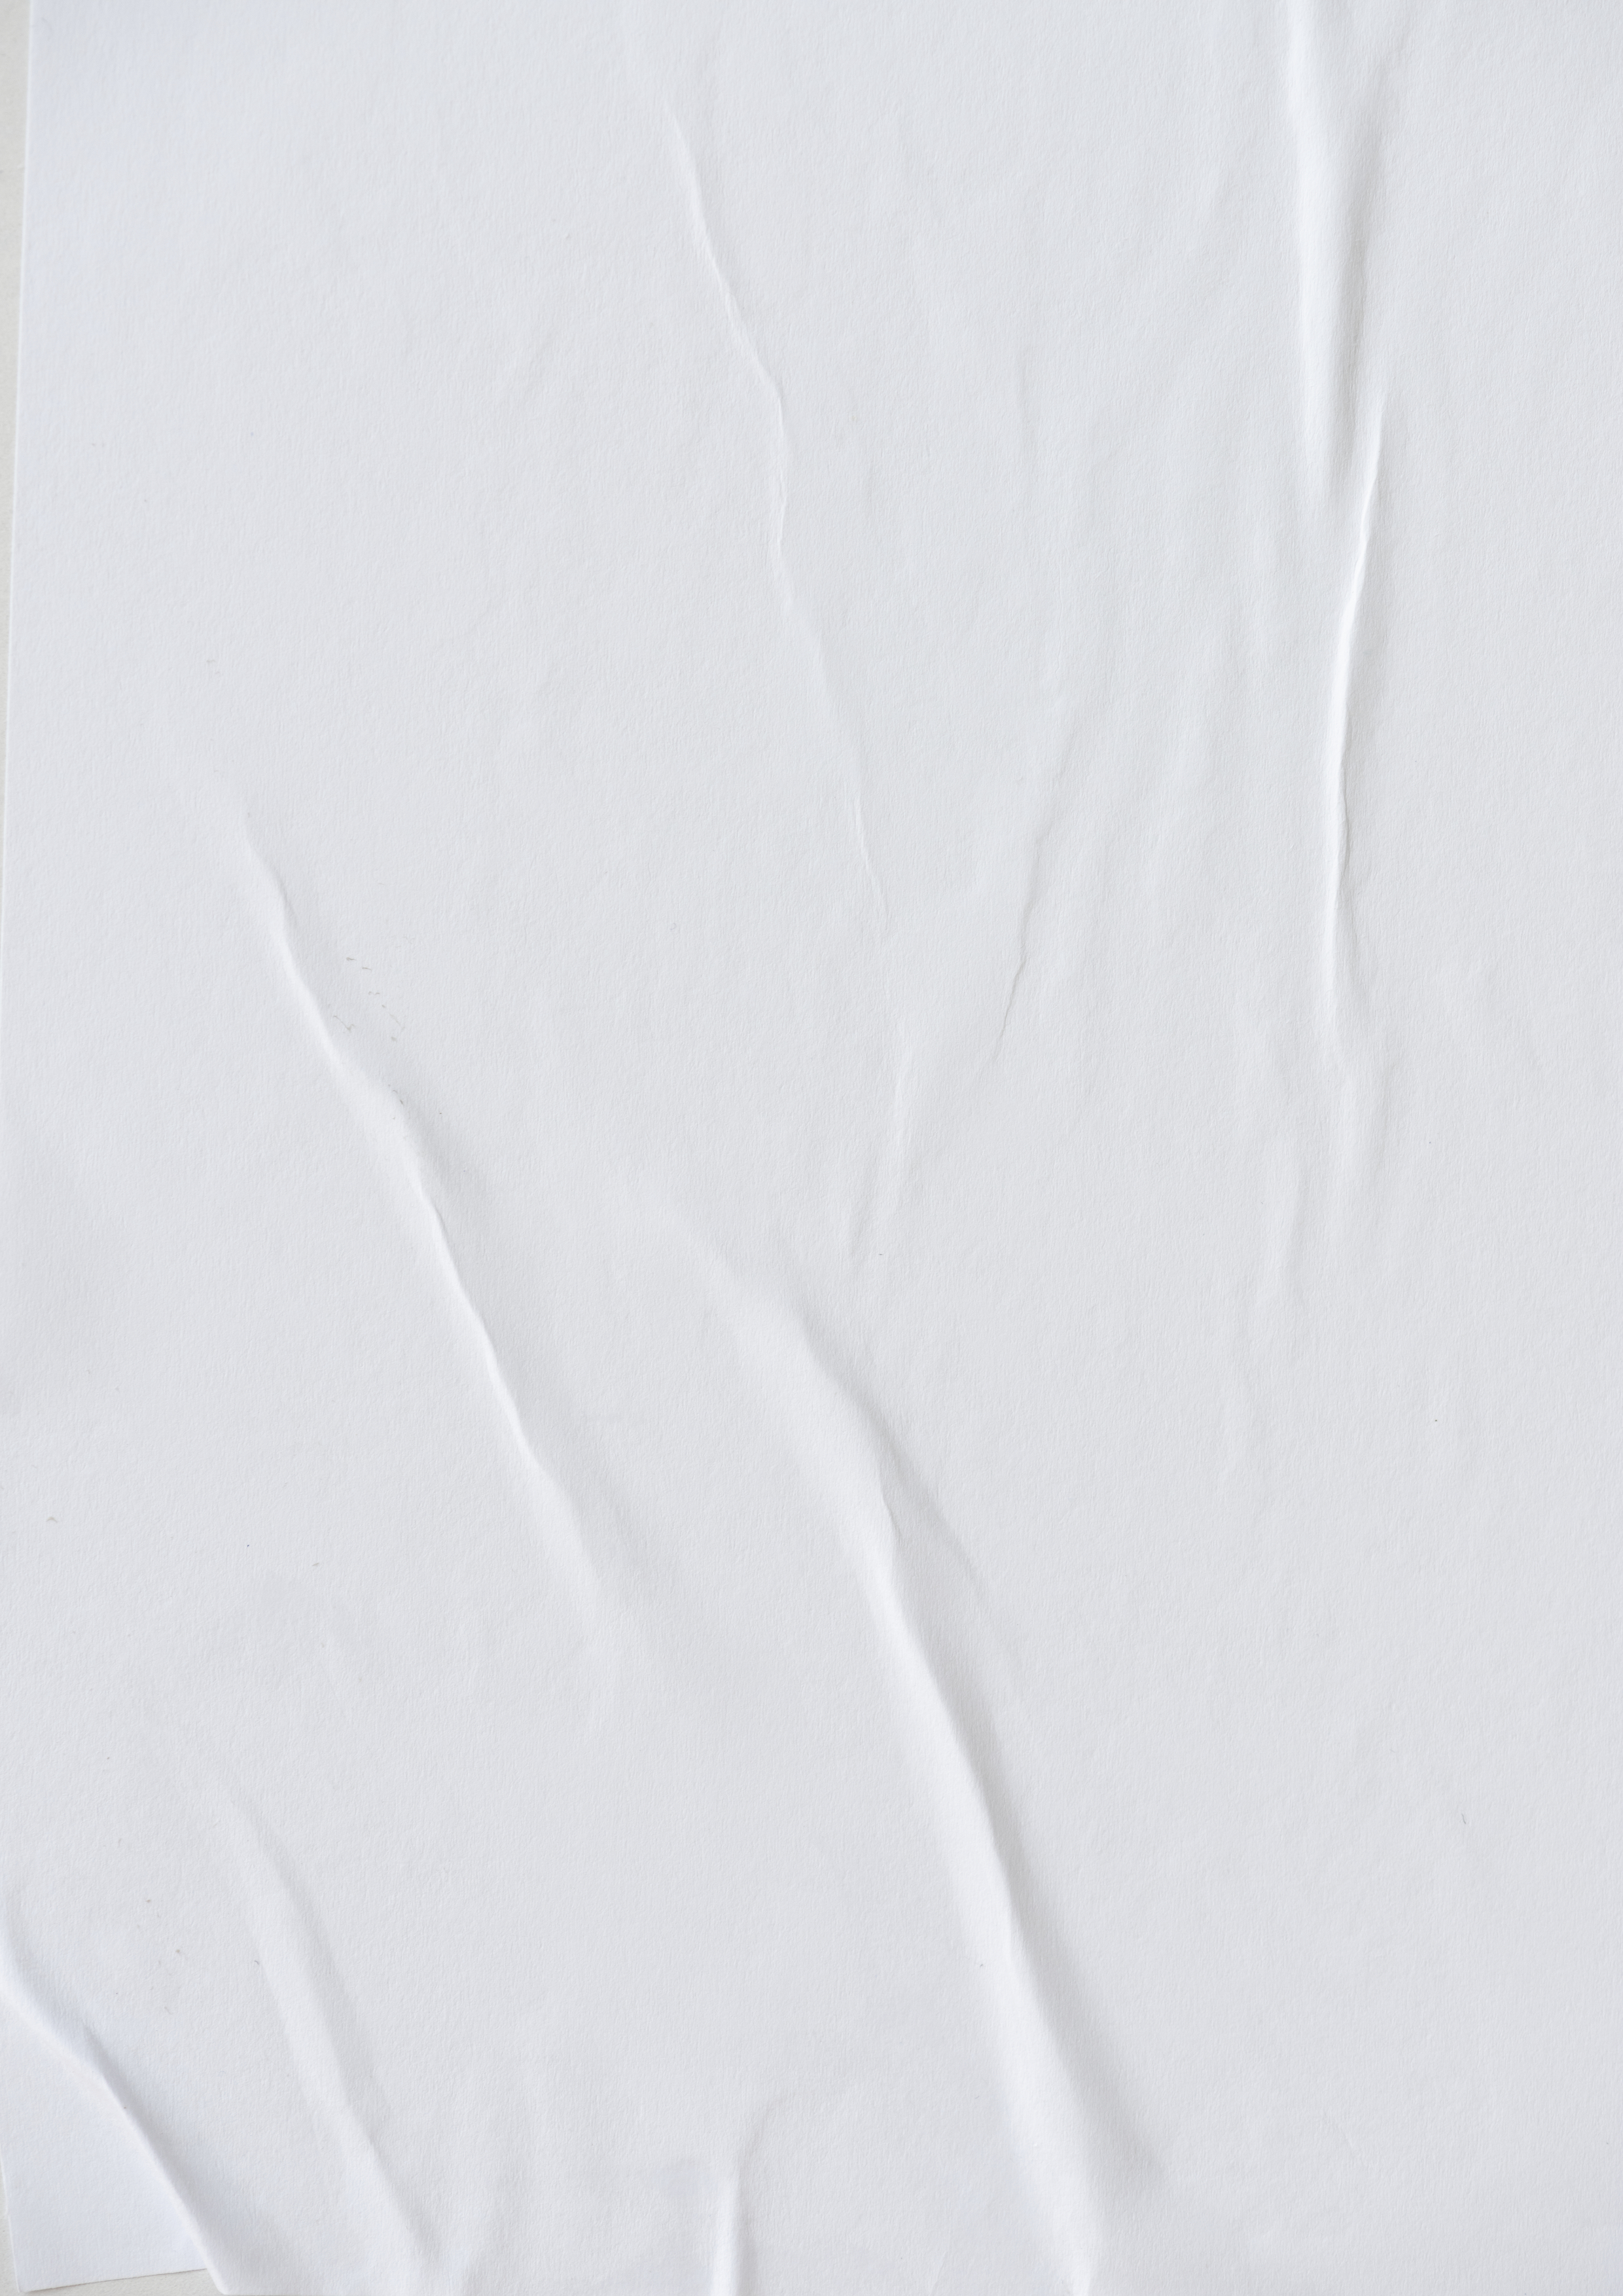
\includegraphics[width=\textwidth]{images/004.jpg}
        \caption{Slight creases.}
    \end{subfigure}
    \begin{subfigure}{0.3\textwidth}
        \includegraphics[width=\textwidth]{images/009.jpg}
        \caption{Moderate crumpling.}
    \end{subfigure}
    \begin{subfigure}{0.3\textwidth}
        \includegraphics[width=\textwidth]{images/005.jpg}
        \caption{Severe wrinkling.}
    \end{subfigure}
    \caption{Examples of crumpled and scratched paper with increasing intensity.}\label{fig:creased-paper}
\end{figure}

Smudges and blurring effects introduce soft, unpredictable distortions, altering the paper's texture. As shown in Figure~\ref{fig:smudged-paper}, these variations create areas of differing opacity and contrast, mimicking the imperfections found in real-world printed materials.

\begin{figure}
    \centering
    \begin{subfigure}{0.3\textwidth}
        \includegraphics[width=\textwidth]{images/003.jpg}
        \caption{Minor smudge.}
    \end{subfigure}
    \begin{subfigure}{0.3\textwidth}
        \includegraphics[width=\textwidth]{images/002.jpg}
        \caption{Moderate blurring.}
    \end{subfigure}
    \begin{subfigure}{0.3\textwidth}
        \includegraphics[width=\textwidth]{images/001.jpg}
        \caption{Severe distortion.}
    \end{subfigure}
    \caption{Examples of blurring and distortion with increasing intensity.}\label{fig:smudged-paper}
\end{figure}

\subsection{Icon Integration and Blending Process}

To integrate the icon into the selected texture, a random texture $T$ is first selected from the \texttt{texture\_pack} directory. The algorithm then computes a height map $H$ from the chosen texture. This map represents variations in the surface texture and is derived by first converting the texture to grayscale and then normalizing its pixel values:
\begin{equation}
    H(x, y) = \frac{T_{gray}(x, y) - \min(T_{gray})}{\max(T_{gray}) - \min(T_{gray})} \times 255.
\end{equation}
This ensures that the values range from 0 (darkest regions) to 255 (brightest regions), allowing for consistent degradation modeling.

Next, the icon is randomly positioned within the texture to simulate natural placement:
\begin{equation}
    x_0 \sim U(0, W_T - W_I), \quad y_0 \sim U(0, H_T - H_I),
\end{equation}
where $W_T, H_T$ are the dimensions of the texture and $W_I, H_I$ are the dimensions of the icon.

The degradation effect is applied using a visibility factor $\alpha$, which is randomly sampled within a predefined range:
\begin{equation}
    \alpha \sim U(\alpha_{min}, \alpha_{max}).
\end{equation}
Using this factor, a degradation map $D$ is constructed from the corresponding height map region:
\begin{equation}
    D(x, y) = \left(1 - \frac{H(x_0 + x, y_0 + y)}{255}\right) \cdot \alpha.
\end{equation}
This equation ensures that higher regions in the height map contribute to stronger degradation effects.

The icon itself is then adjusted according to the computed degradation:
\begin{equation}
    I' = I_{gray} \cdot D.
\end{equation}
where $I_{gray}$ represents the grayscale version of the icon, ensuring that degradation uniformly affects its intensity.

If the icon contains an alpha channel $A_I$, it is modified accordingly:
\begin{equation}
    A'_I = A_I \cdot D.
\end{equation}
This step ensures that transparency levels are also affected by the degradation process.

Finally, the blended image $B$ is constructed by merging the degraded icon with the texture background using alpha compositing:
\begin{equation}
    B(x, y) = I'(x, y) \cdot A'_I(x, y) + T(x_0 + x, y_0 + y) \cdot (1 - A'_I(x, y)).
\end{equation}


After blending, a windowed extraction is performed to crop a region around the icon, incorporating additional padding to maintain a realistic blend with the background. The cropping boundaries are determined as:
\begin{equation}
    x_{\min} = \max(0, x_0 - B_W), \quad x_{\max} = \min(W_T, x_0 + W_I + B_W)
\end{equation}
\begin{equation}
    y_{\min} = \max(0, y_0 - B_H), \quad y_{\max} = \min(H_T, y_0 + H_I + B_H)
\end{equation}
where the final extracted image contains both the icon and additional background, preserving the natural degradation effect.

\subsection{Implementation Details}

The method is implemented using OpenCV and NumPy to efficiently perform image transformations and blending operations. The algorithm dynamically selects textures from the \texttt{texture\_pack} directory, ensuring a variety of degradation patterns. The randomized positioning and degradation factors ensure that each augmented image exhibits unique characteristics, enhancing dataset diversity for robust training applications.
